\documentclass[12pt]{article}
\usepackage[margin=2cm]{geometry}
\usepackage{titling}
\usepackage{graphicx}
\usepackage{float}
\usepackage[hidelinks]{hyperref}
\usepackage[italian]{babel}
\usepackage{subcaption}

\setlength\parindent{0pt}
\setlength{\parskip}{1em}
\setlength{\droptitle}{-2cm}

\title{Istruzioni d'uso TableFootballPlus}
\author{Università della Svizzera Italiana}
\date{Versione \today}


\begin{document}
\maketitle
\tableofcontents
\newpage

\section{Montaggio}

	\subsection{Montaggio}

		//TODO
		
		

\section{Utilizzo}

	Per iniziare a giocare, collegare la presa di corrente e aspettare qualche secondo. Dopo il tono di avvio, il tavolo sarà pronto all'uso.
	
	Ad ogni goal segnato, il tavolo si illuminerà brevemente con il colore della squadra corrispondente. Quando una delle due squadre raggiunge la vittoria (10 punti), il colore corrispondente lampeggia in continuo e i goal non saranno più conteggiati. È possibile annullare la vittoria in caso di un errore (vedi sotto).
	
	Per aggiustare manualmente il punteggio (in caso di errori di rilevamento), su ogni lato sono disponibili dei pulsanti per incrementare (\texttt{+}) o decrementare (\texttt{-}) manualmente il punteggio.
	
	Per cominciare una nuova partita, premere il tasto rosso (\texttt{Restart}).
	
	Per cambiare il colore o spegnere le luci, premere il tasto blu (\texttt{Lights}).
	
	\begin{figure}[H]
        \begin{subfigure}{0.5\textwidth}
                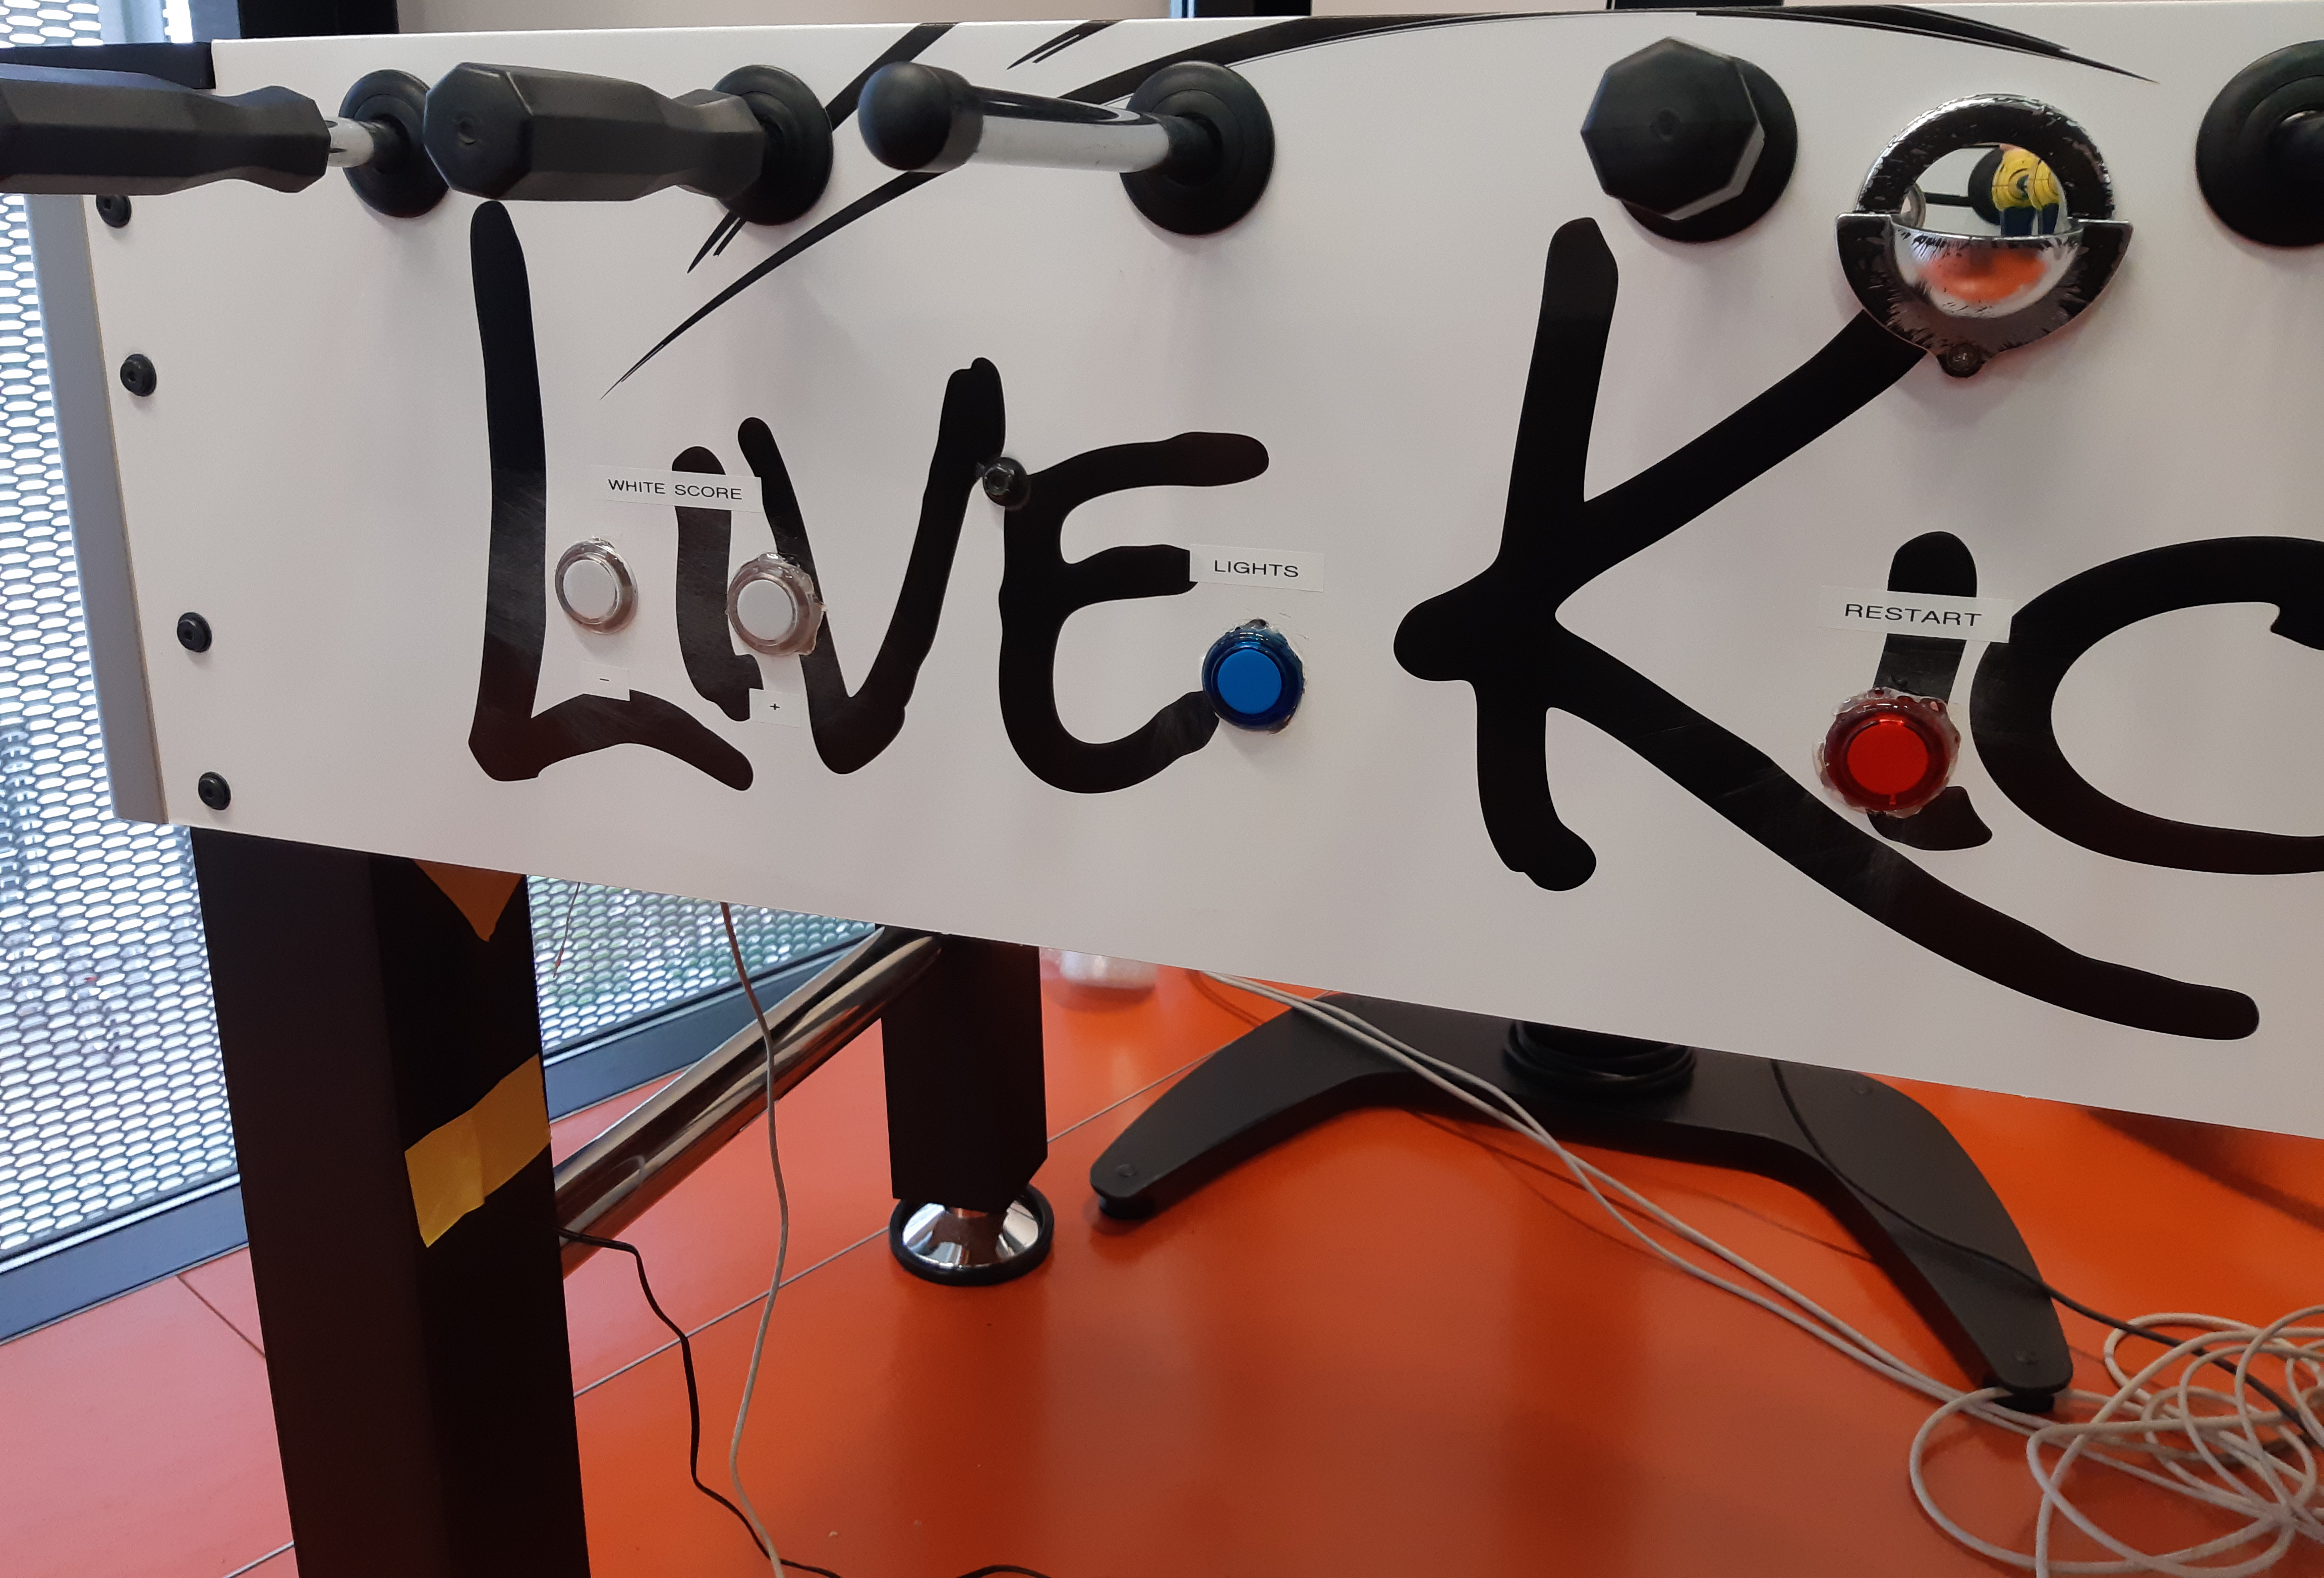
\includegraphics[width=0.9\textwidth]{img/btn_white.jpg}
                \caption*{I pulsanti per il team bianco}
        \end{subfigure}
        \begin{subfigure}{0.5\textwidth}
                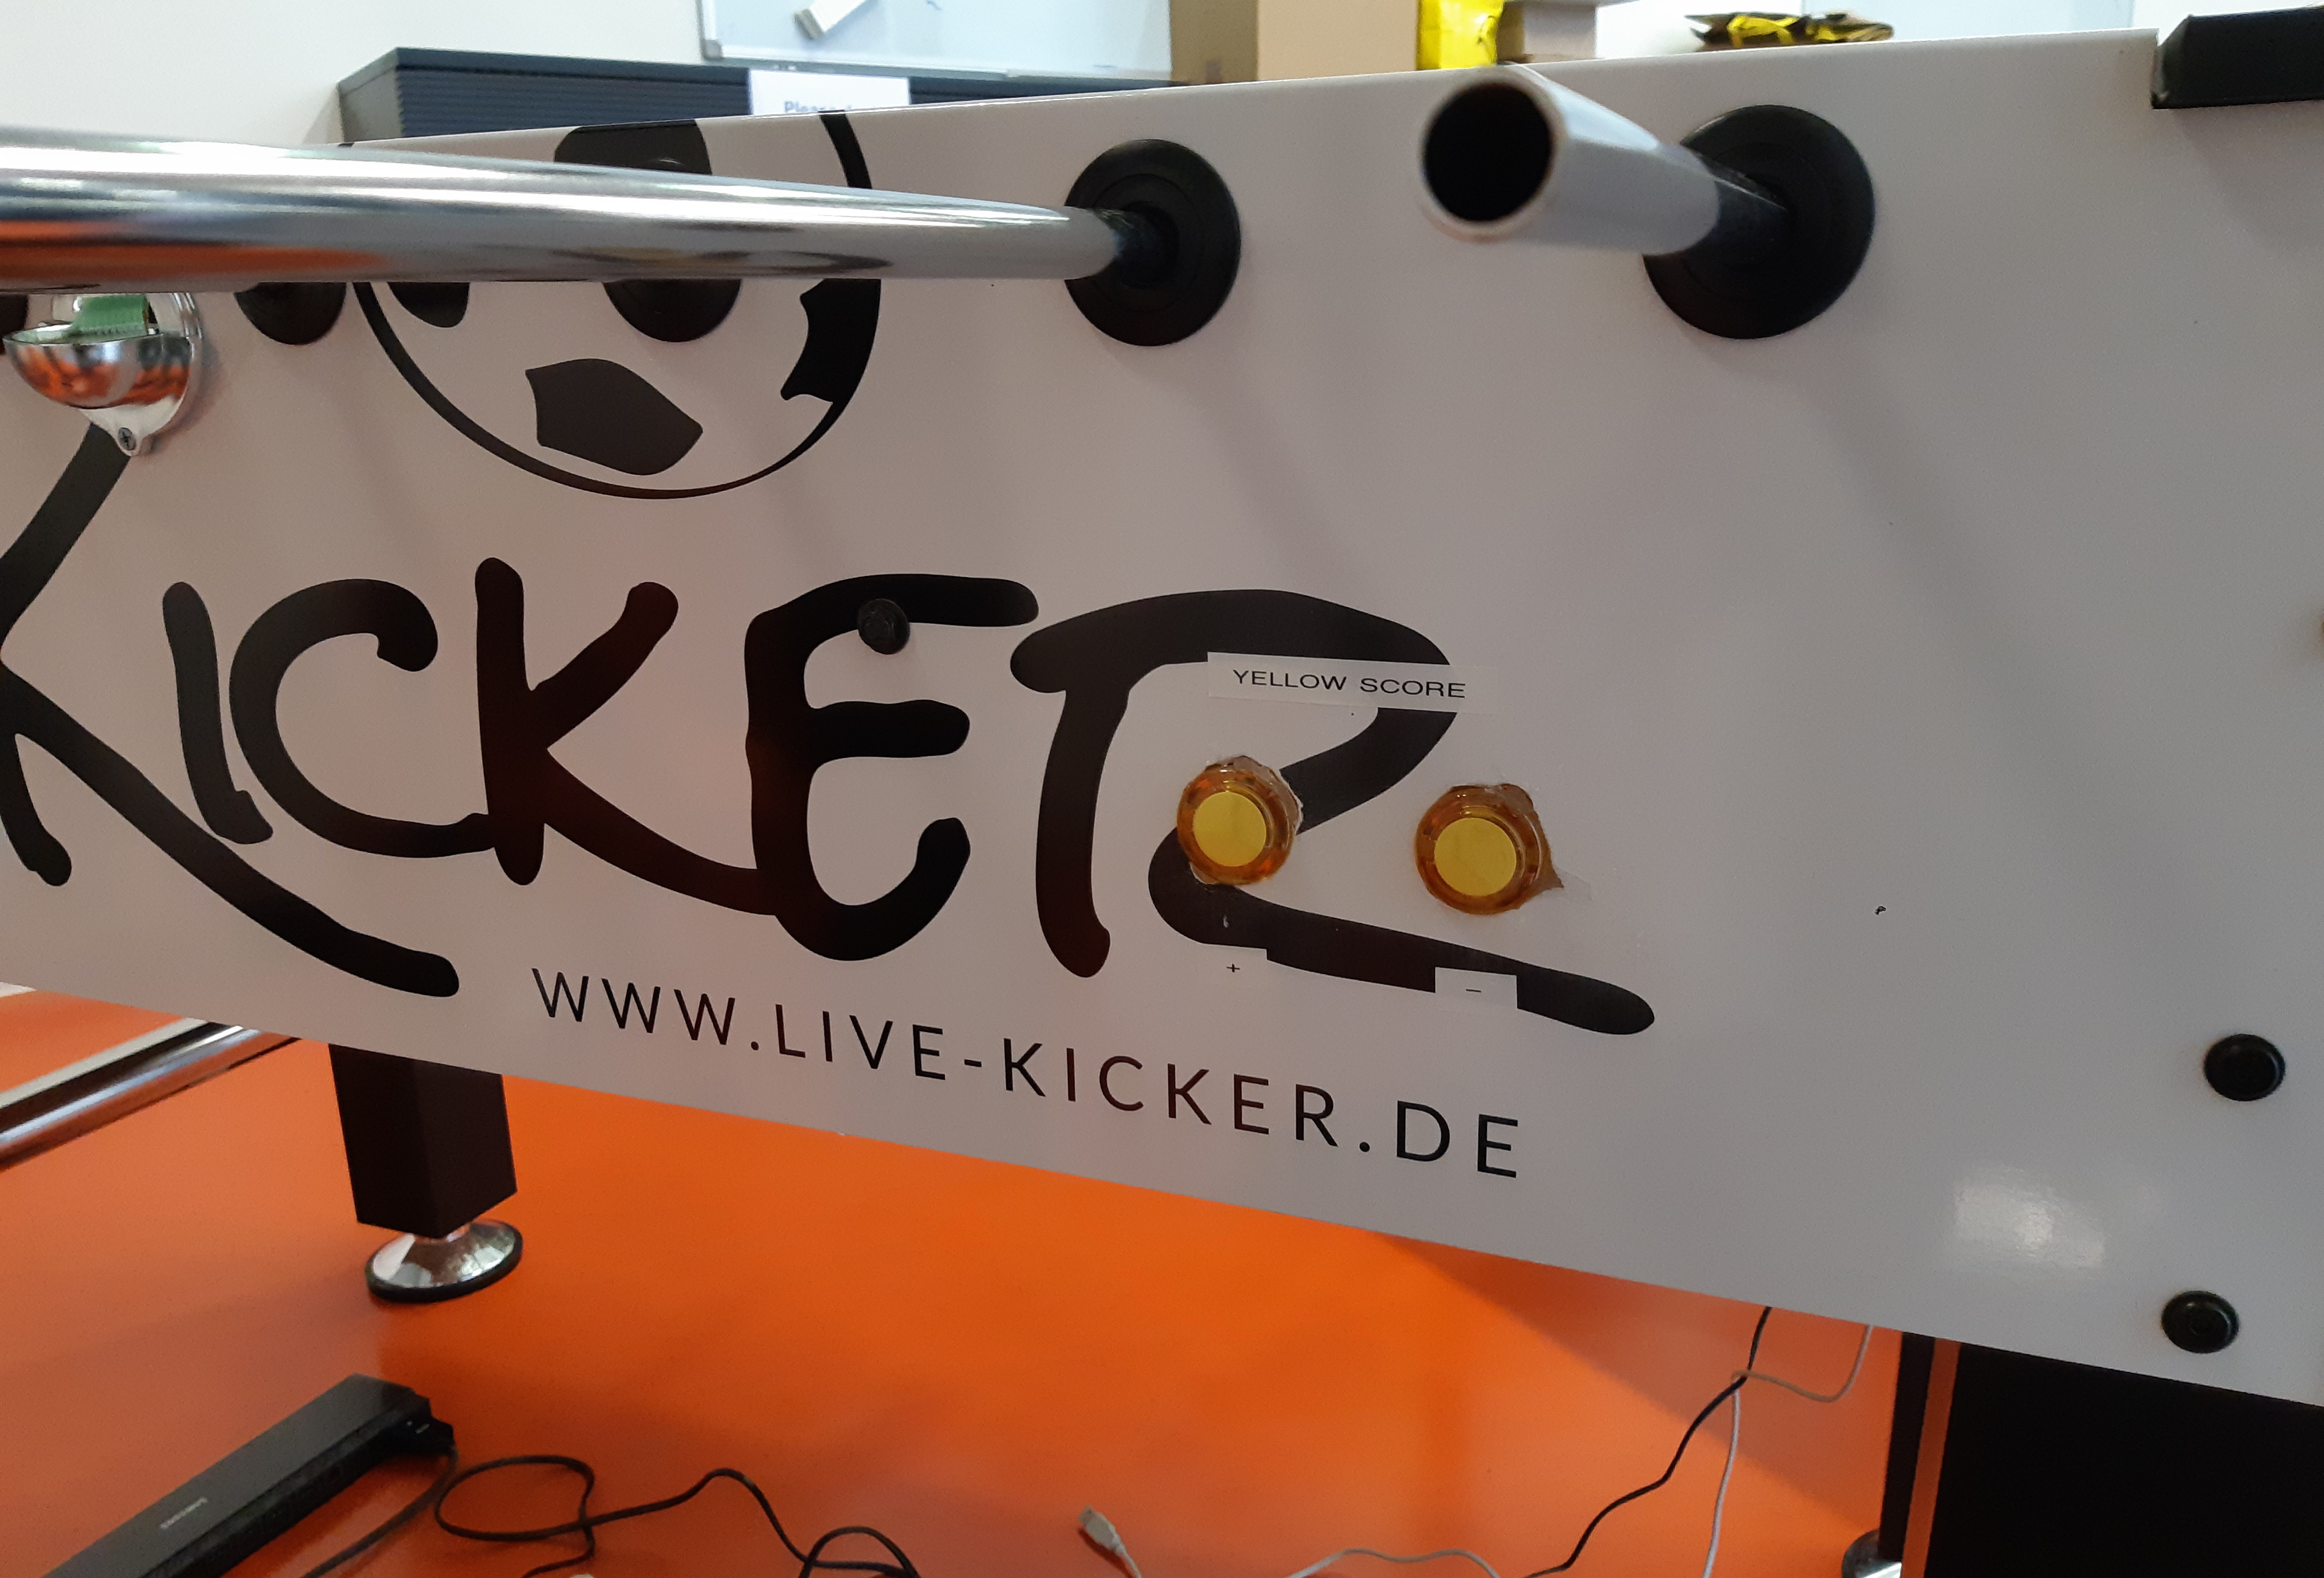
\includegraphics[width=0.9\textwidth]{img/btn_yellow.jpg}
                \caption*{I pulsanti per il team giallo}
         \end{subfigure}
	\end{figure}
	
	
	
\section{Circuito}

	Di seguito è una rappresentazione schematica del circuito: 
	
	\begin{figure}[H]
                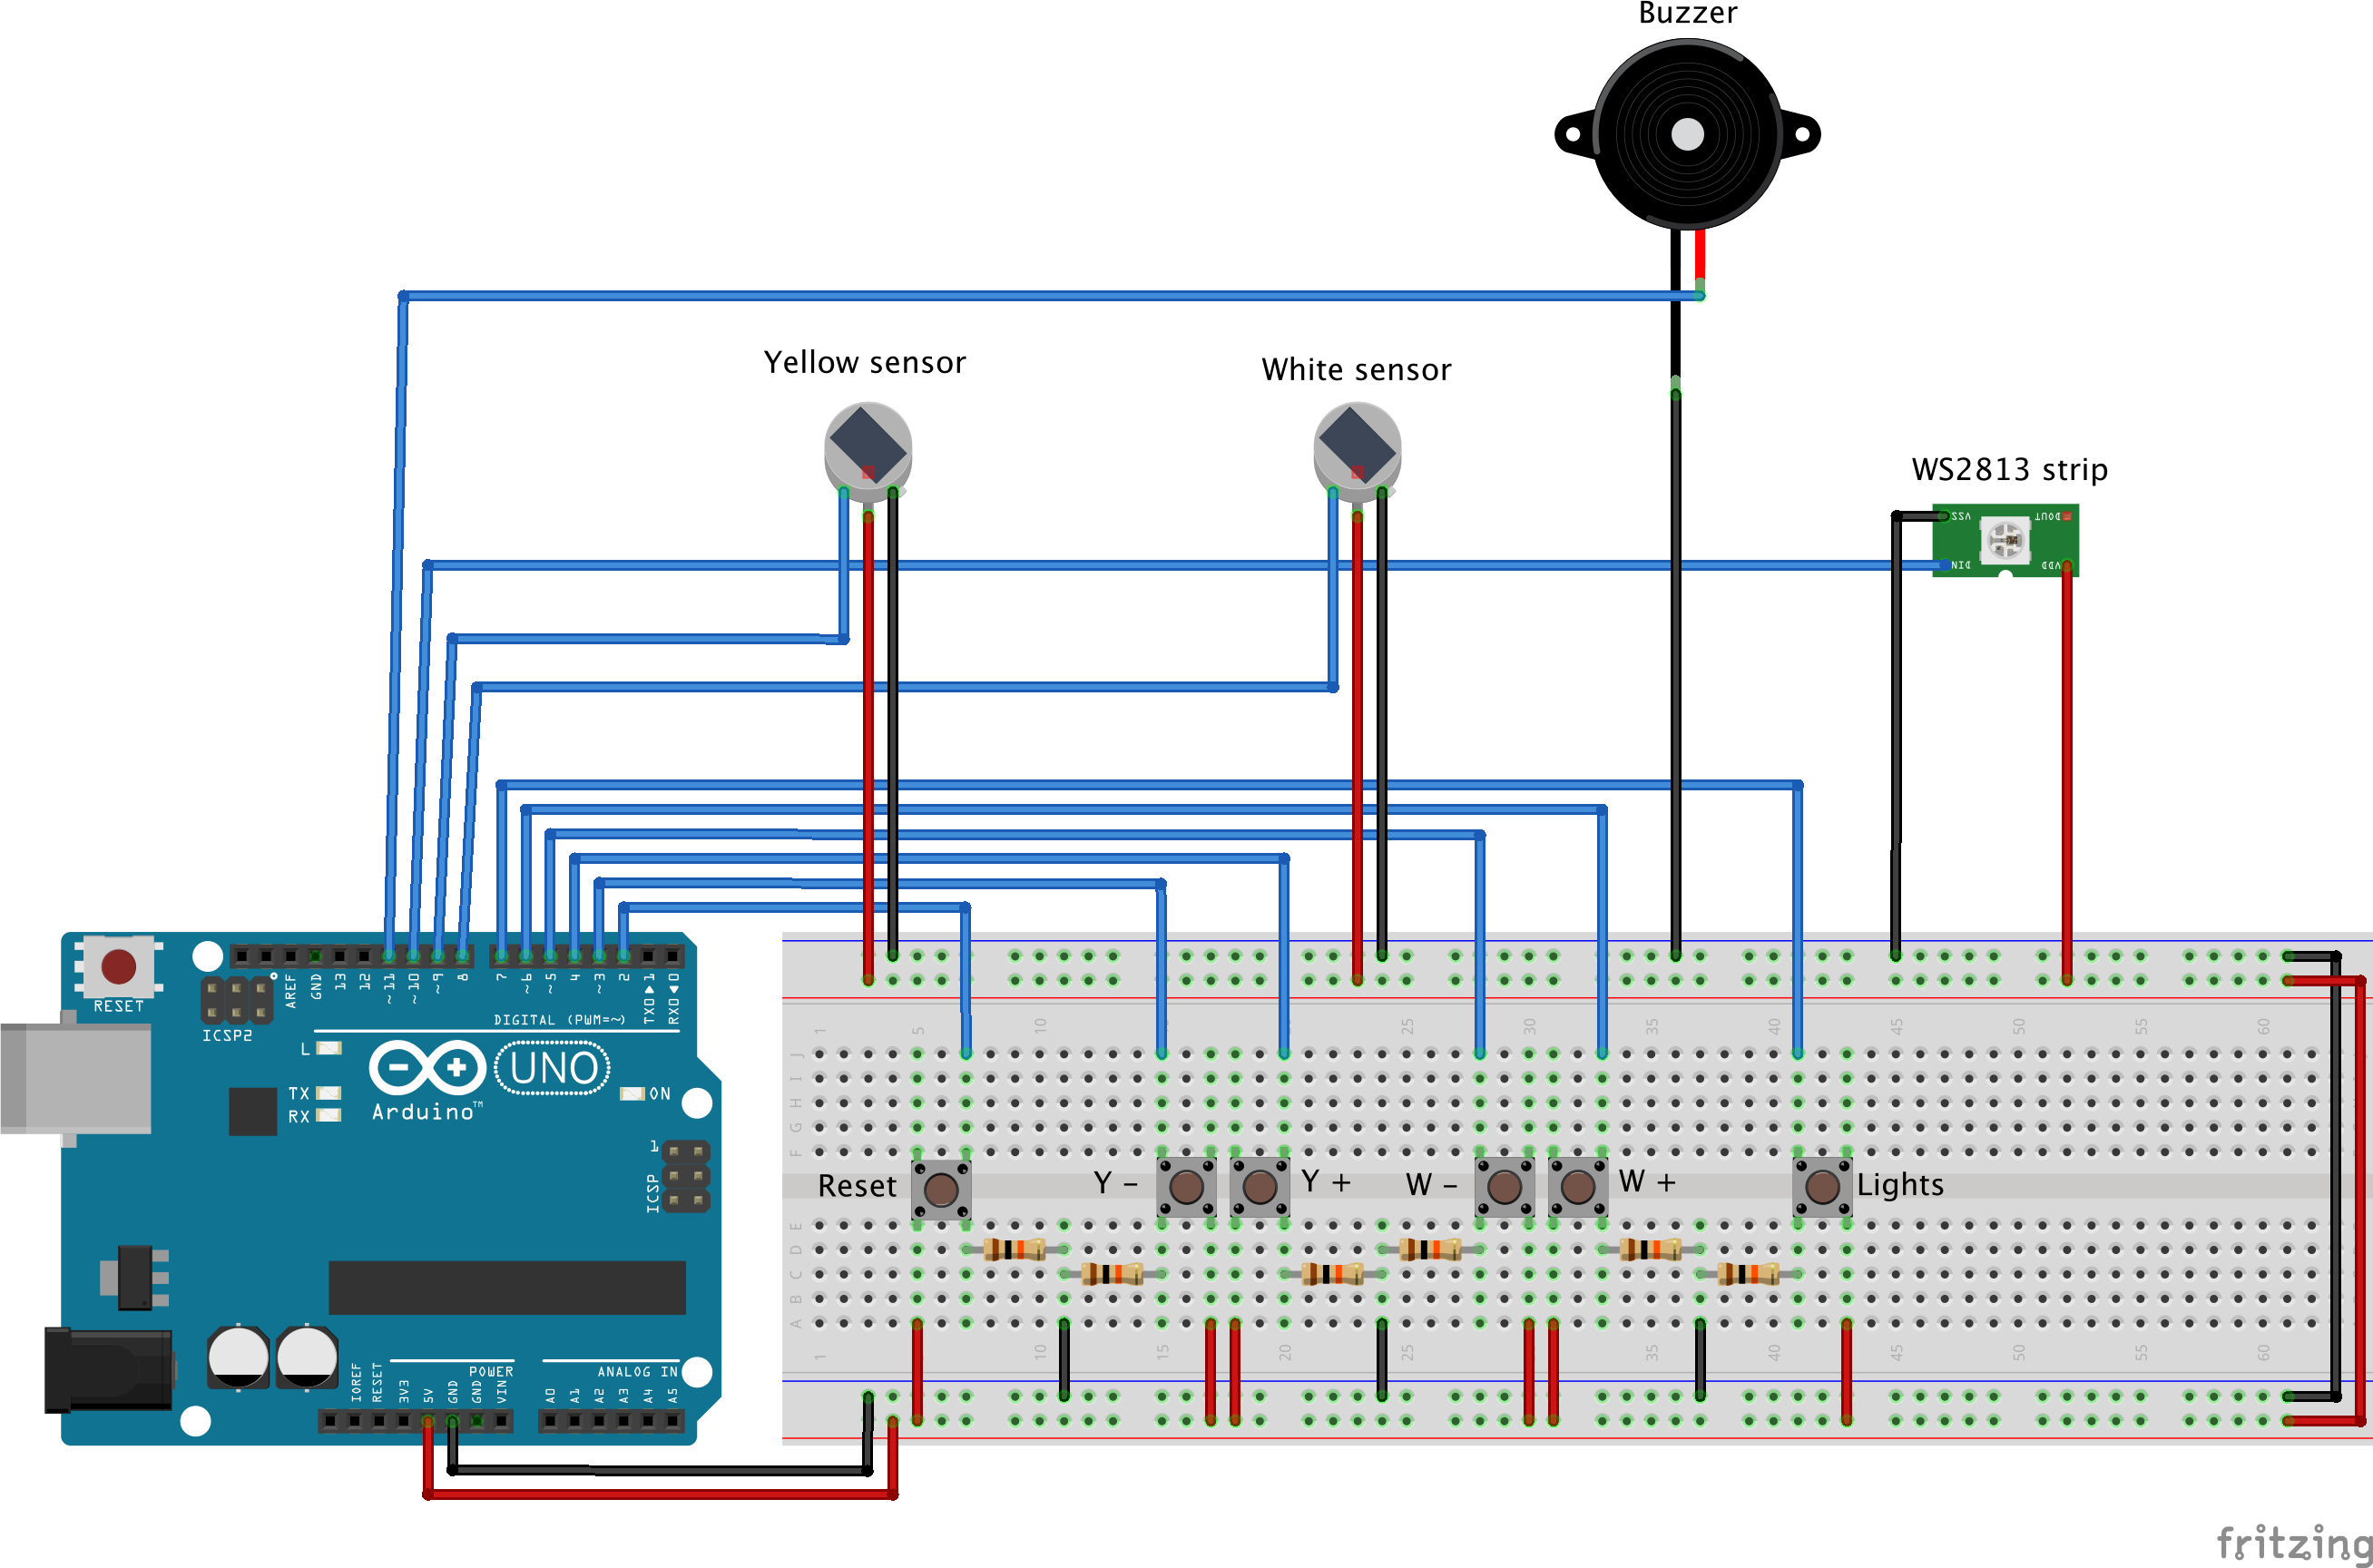
\includegraphics[width=\textwidth]{img/circuit.png}
        \end{figure}
	


\section{Codice}

	Il codice e la presente documentazione si trovano al seguente indirizzo: \url{https://github.com/USI-Showroom/TableFootballPlus}

\end{document}
